\documentclass{article}

\title{Laporan Modul 3}

\author{Jihad Amal Farid NRP 5024211072 \\ Muhammad Firdaus Anvi Putra NRP 5024211067 \\ Muhammad Fathi Farhat NRP 5024211065 \\ Nico Syahrizal Anam NRP 5024211057}

\date{3 Juli 2023}

\usepackage{graphicx}

\begin{document}
    \maketitle
    \section{Pendahuluan}
    Dalam era digital yang semakin berkembang, ketersediaan dan kualitas koneksi internet menjadi sangat penting. Kemampuan untuk mengukur dan memahami kecepatan internet atau bandwidth merupakan faktor krusial dalam menentukan pengalaman pengguna dan keberhasilan berbagai aplikasi dan layanan online.
    
    \section{Tujuan Praktikum}
    Praktikum ini bertujuan untuk membahas tentang pengujian bandwidth, yang merupakan metode untuk mengukur kecepatan dan kualitas koneksi internet. Pengujian bandwidth melibatkan pengiriman dan penerimaan data dalam jaringan dengan tujuan untuk menentukan sejauh mana kinerja koneksi internet dalam menghadirkan kecepatan yang dijanjikan oleh penyedia layanan.
    
    \section{Alat dan Bahan}
    Berikut adalah alat dan bahan untuk praktikum : \\
    1. 1 buah laptop \\ 
    2. 2 buah router \\
    3. 2 kabel LAN \\
    
    \newpage
    \section{Topologi}
    Pada percobaan ini, ether 5 yaitu kabel laptop ke router lalu ether 2 digunakan untuk kabel dari router menuju router induk yaitu router dari ITS. Pada percobaan ini kami hanya menggunakan 1 buah laptop saja.
    \begin{figure}[h!]
        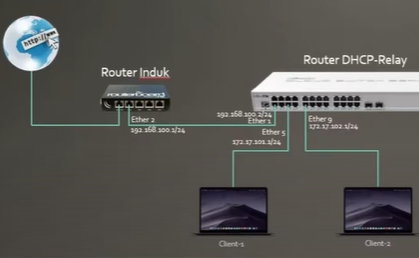
\includegraphics{Topologi.png}
        \caption{Topologi}
    \end{figure}

    \section{Langkah Percobaan}
    \paragraph{}
    A. Konfigurasi DHCP Relay \\
    1. setting ip untuk ether 5 yaitu 172.17.101.1/24 \\ 
    2. buat DHCP Server dengan Interfacenya Ether 2 (router induk ke router DHCP)  dan relaynya adalah 172.17.101.1 \\
    3. buat DHCP network, sesuai network clientnya.\\
    4. buat DHCP Relay dengan interface yang terhubung router induk dan DHCP servernya adalah alamat router induk 192.168.100.1 dan local address adalah alamat IP dari interface yang terhubung dengan client.\\
    \paragraph{}
    B. Setting limit bandwith \\
    1. buka menu bandwith test \\
    2. parameter test to diisi alamat router induk dengan protocol udp \\
    3. isilah local Tx speed dan remote Tx speed sesuai ingin berapa delimit kecepatan internetnya. \\

    \newpage
    \section{Hasil Percobaan}
    \begin{figure}[h!]
        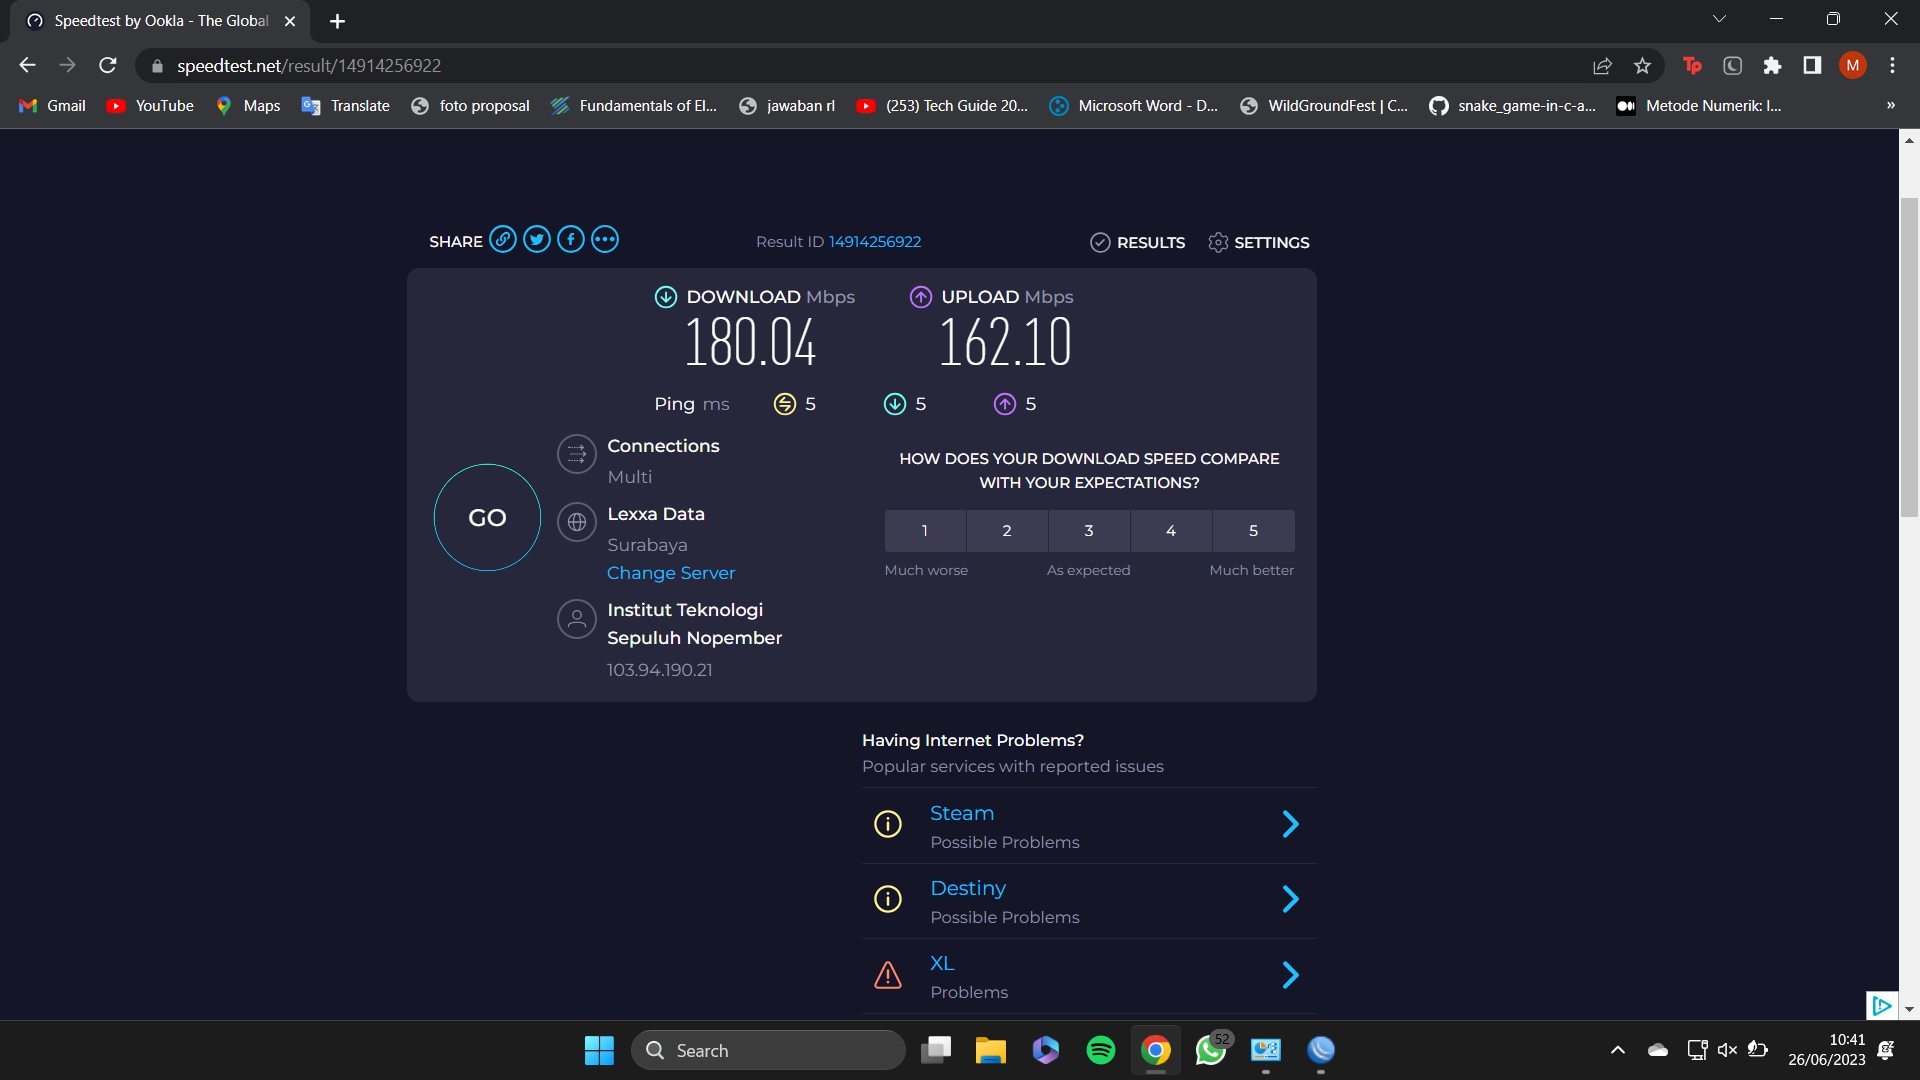
\includegraphics[width=\linewidth]{Before.png}
        \caption{Sebelum dilimit}
    \end{figure}
    \begin{figure}[h!]
        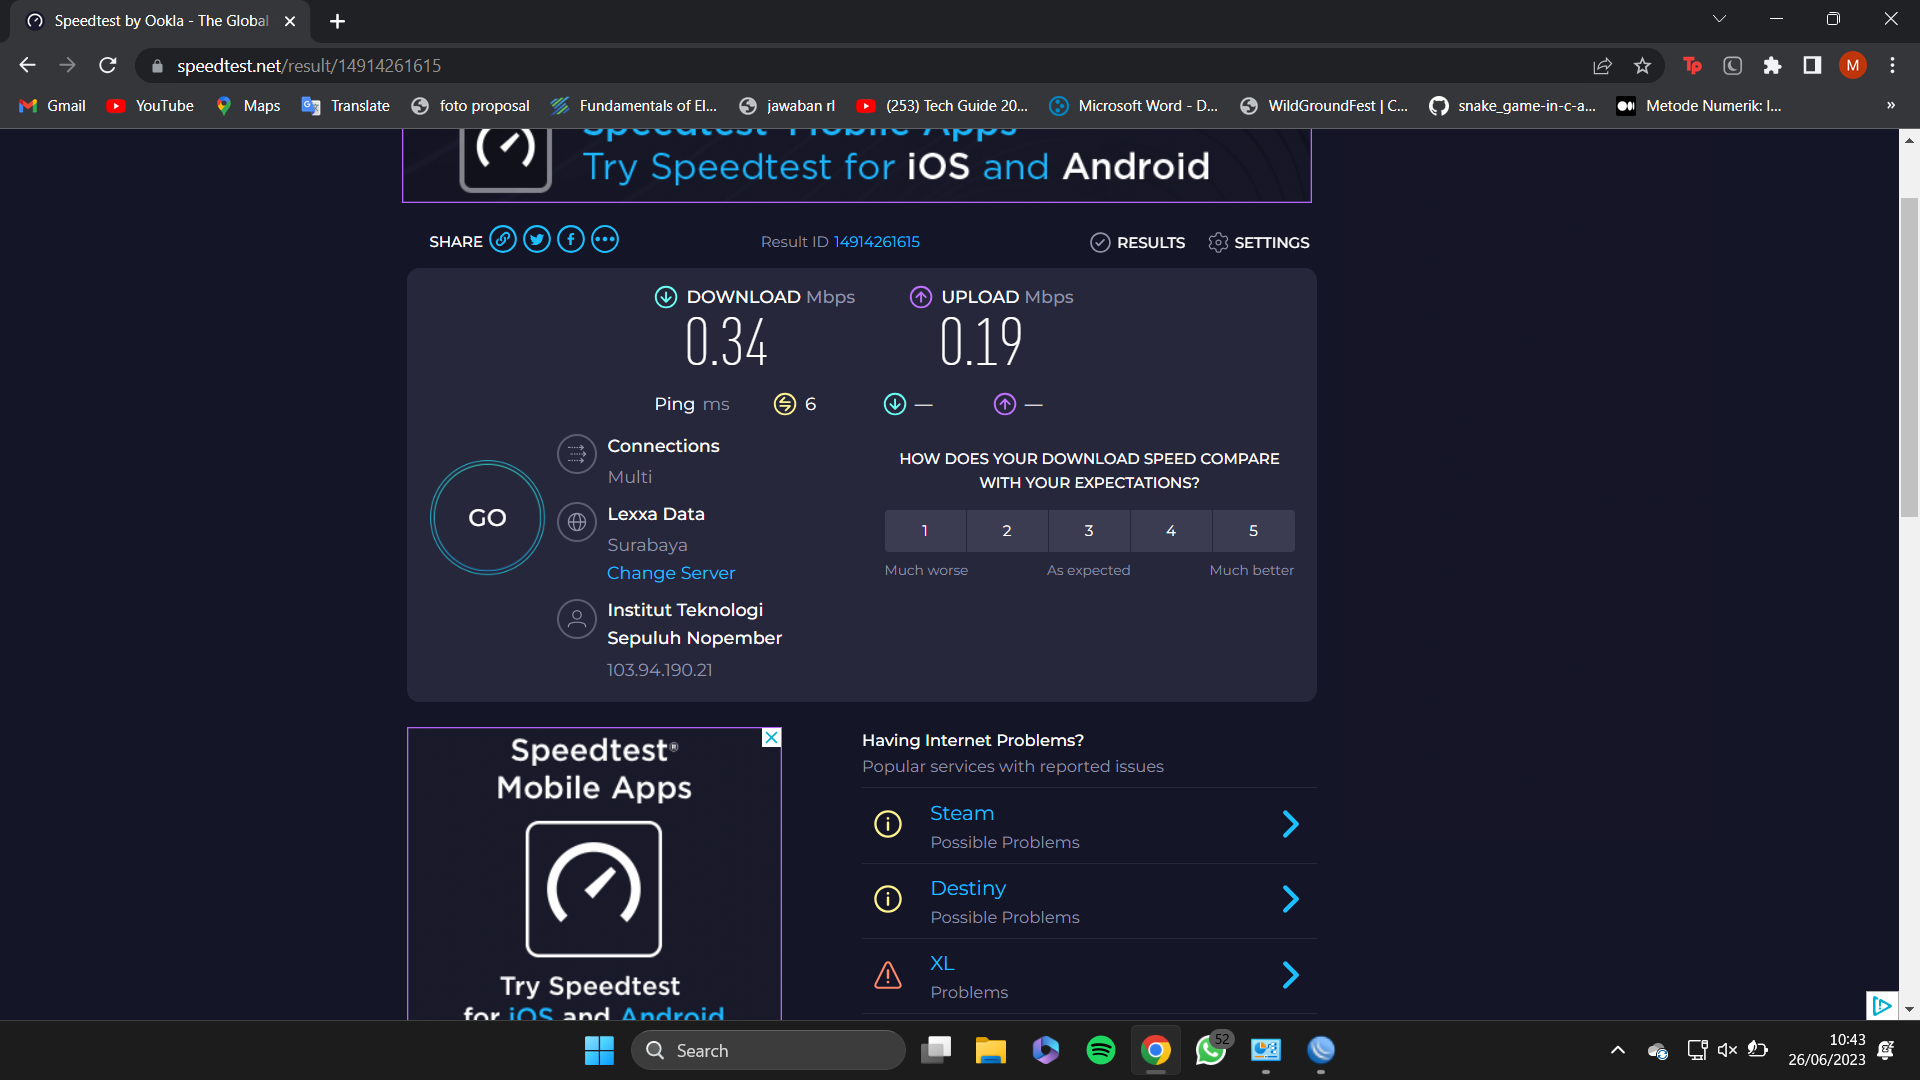
\includegraphics[width=\linewidth]{After.png}
        \caption{Sesudah dilimit}
    \end{figure}

    \newpage
    \section{Kesimpulan}
    Kesimpulan dari praktikum ini adalah cara untuk menghubungkan laptop dengan router menggunakan DHCP dan juga mengetahui cara untuk melimit kecepatan internet.
    \section{Lampiran}
    \begin{figure}[h!]
        \centering
        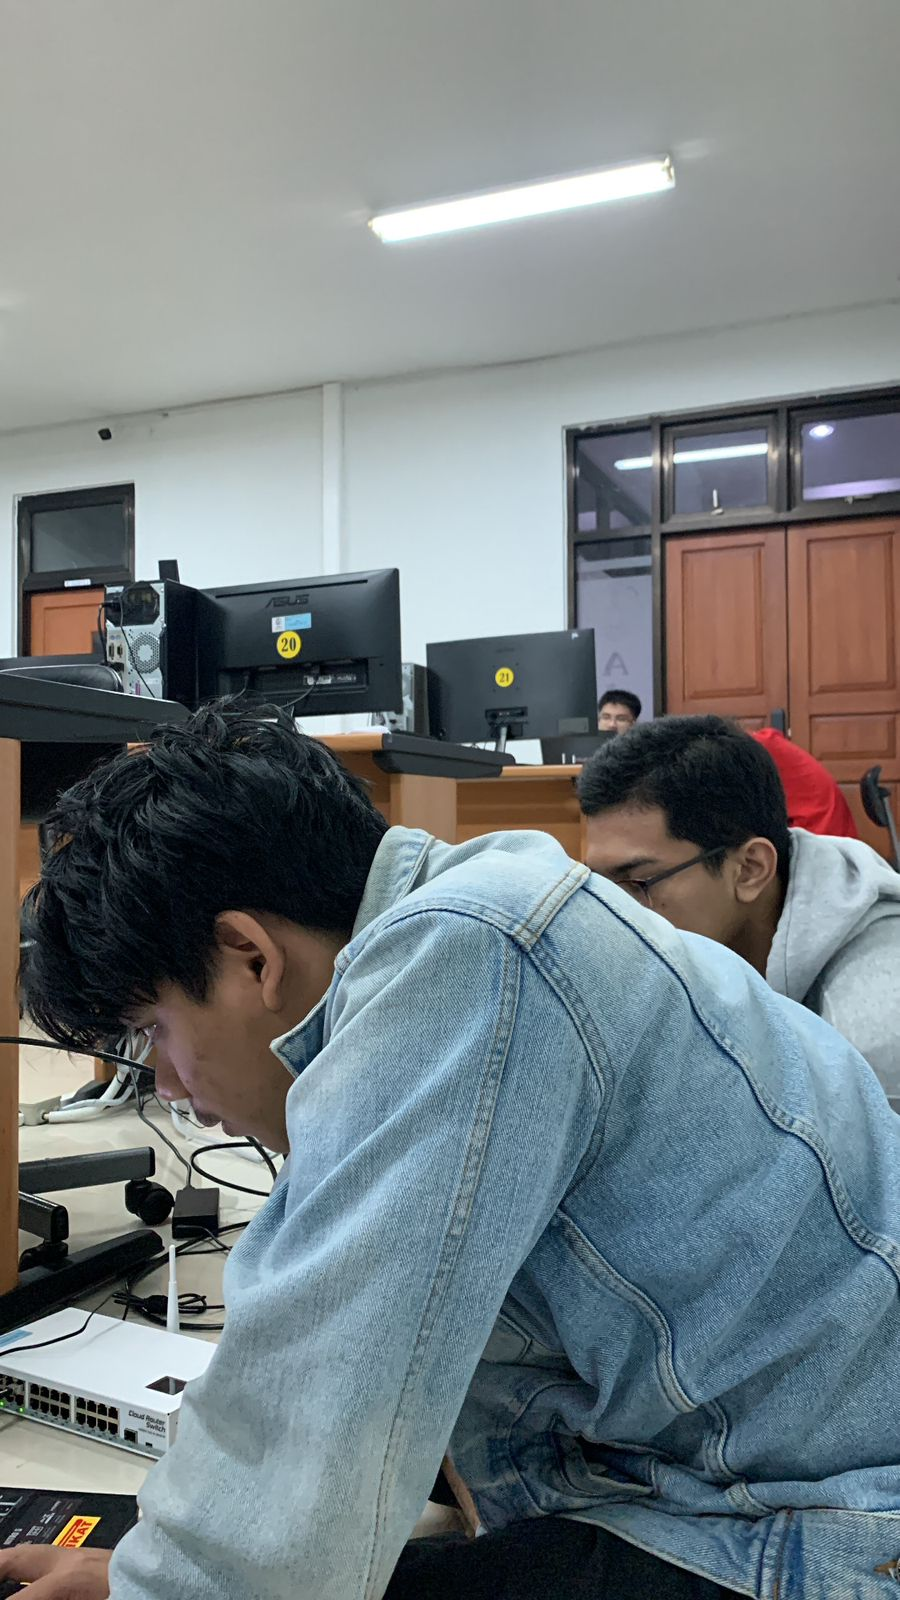
\includegraphics[width=0.3\linewidth]{Kelompok.jpeg}
        \caption{Foto sedang mengerjakan}
    \end{figure}
    \begin{figure}[h!]
        \centering
        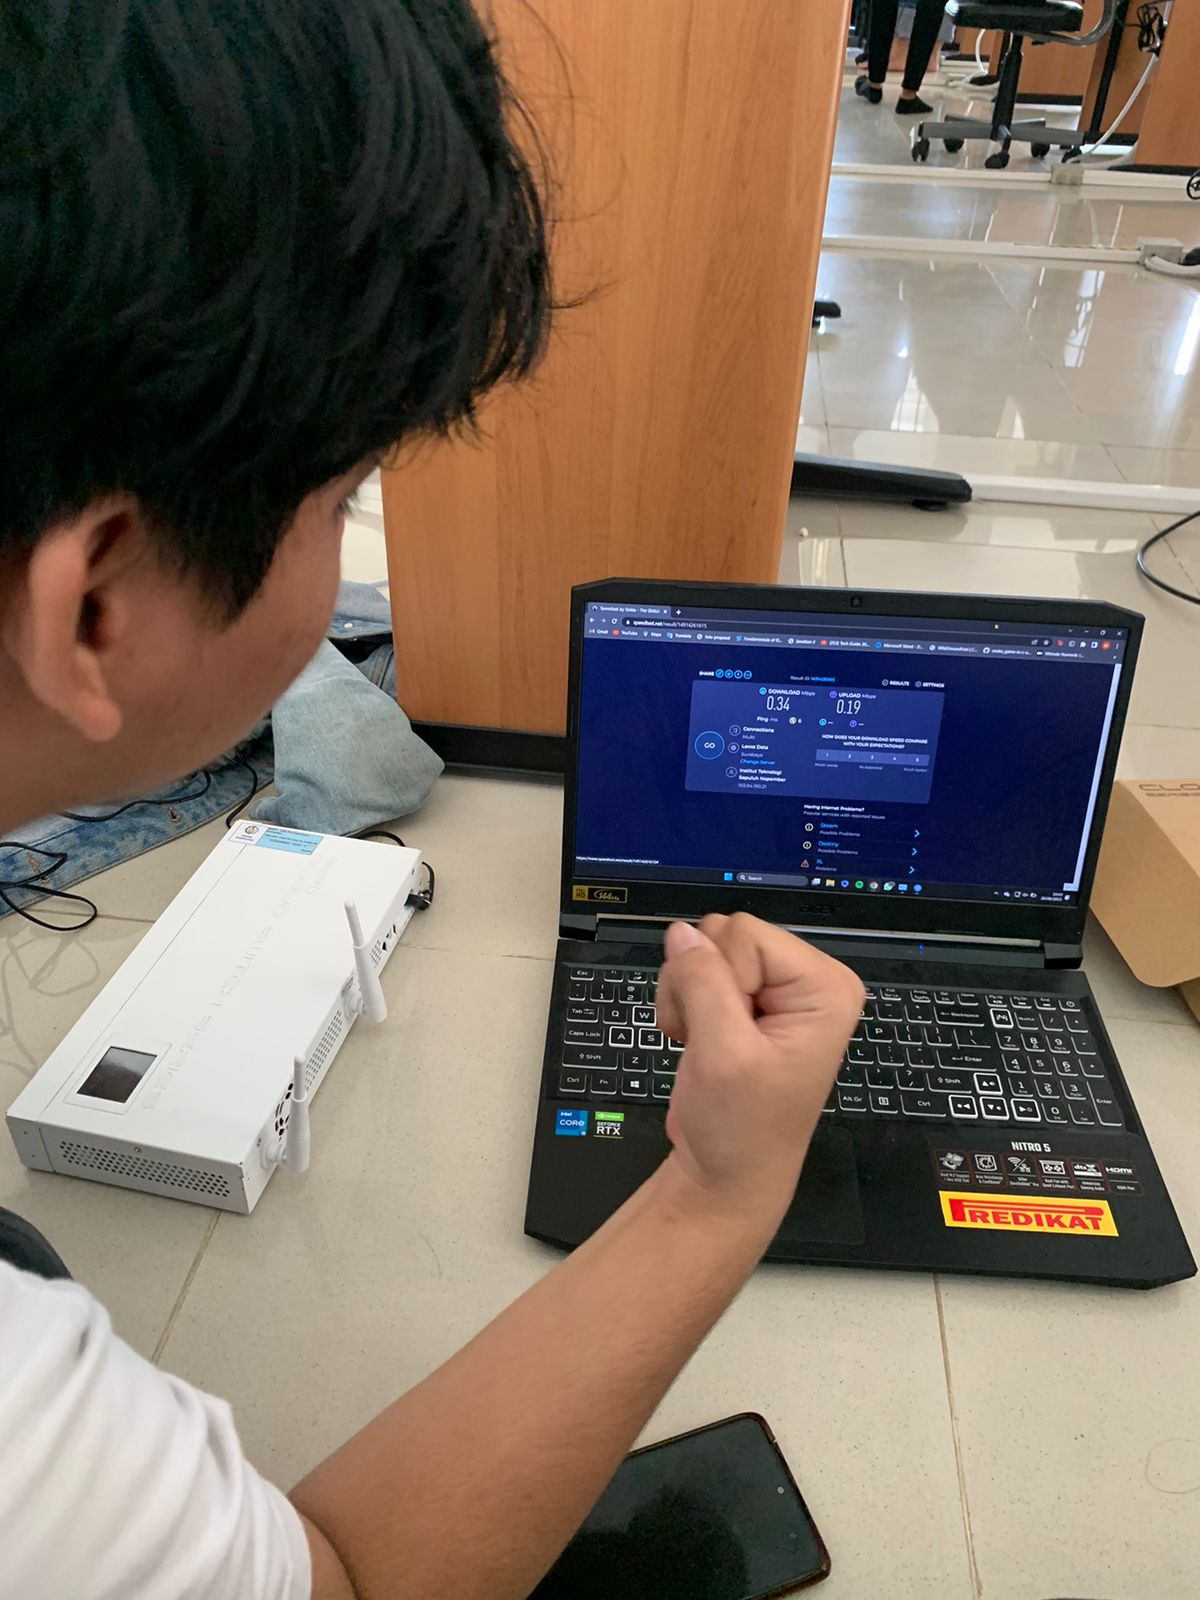
\includegraphics[width=0.35\linewidth]{Done.jpeg}
        \caption{Foto Router dan Laptop}
    \end{figure}
\end{document}